% !TeX spellcheck = en_GB
%%%%%%%%%%%%%%%%%%%%%%%%%% phdsymp_sample2e.tex %%%%%%%%%%%%%%%%%%%%%%%%%%%%%%
%% changes for phdsymp.cls marked with !PN
%% except all occ. of phdsymp.sty changed phdsymp.cls
%%%%%%%%%%              %%%%%%%%%%%%%
%%%%%%%%%% More information: see the header of phdsymp.cls %%%%%%%%%%%%%
%%%%%%%%%%              %%%%%%%%%%%%%
%%%%%%%%%%%%%%%%%%%%%%%%%%%%%%%%%%%%%%%%%%%%%%%%%%%%%%%%%%%%%%%%%%%%%%%%%%%%%%%


\documentclass[twocolumn]{phdsymp} %!PN

\usepackage[dutch]{babel}  % Voor nederlandstalige hyphenatie (woordsplitsing)

\usepackage{graphicx}     % Om figuren te kunnen verwerken
\usepackage{graphics}			% Om figuren te verwerken.

\graphicspath{images/}

\PassOptionsToPackage{hyphens}{url}
\usepackage{url}

\usepackage[T1]{fontenc}

\usepackage{amsmath}
\usepackage{packages/customcommands}

\hyphenation{}

\def\BibTeX{{\rm B\kern-.05em{\sc i\kern-.025em b}\kern-.08em
 T\kern-.1667em\lower.7ex\hbox{E}\kern-.125emX}}

\newtheorem{theorem}{Theorem}

\begin{document}

\title{Client-side evaluatie van GeoSPARQL opvragingen over heterogene gegevensbronnen} %!PN

\author{Andreas De Witte}

\supervisor{dr. ing. Pieter Colpaert, dr. ir. Ruben Taelman, Brecht Van de Vyvere, Julian Andres Rojas Melendez}

\maketitle

\begin{abstract}
    Op het Web zoals het nu gekend is, kunnen gebruikers makkelijk pagina's van websites begrijpen. Voor computers is dit echter niet het geval, hier moet enorm veel moeite gedaan worden om betekenis en context uit de zinnen te ontleden. Het Web zoals het nu is, is niet gebouwd om begrepen te worden door machines. Dankzij het Semantische Web, wat een uitbreiding op het huidige Web is, is het wel mogelijk voor machines om de pagina's van websites te begrijpen.
    
    Momenteel is het reeds mogelijk om opzoekingen naar gelinkte data te doen over een beperkt aantal gegevensbronnen, omdat weinig gegevensbronnen gelinkte data ondersteunen. Deze gegevensbronnen kunnen ook heterogeen zijn, wat betekent dat het andere types van bronnen kunnen zijn. Deze opzoekingen gebeuren aan de hand van SPARQL, waar verschillende werkende implementaties van zijn. Om geografische opvragingen te doen wordt GeoSPARQL gebruikt. Hiervan zijn echter weinig implementaties gemaakt en deze implementaties hebben in vele gevallen incorrecte gedragingen.
    
    In dit werk is een beperkte implementatie van GeoSPARQL gemaakt om zo de informatie in RDF formaat op te halen en topologische relaties uit te rekenen. Hierbij is getest bij welk soorten interfaces deze topologische relaties op de client-side kunnen worden berekend. Dit op de client-side doen is belangrijk voor vele redenen. Eén van de belangrijkste redenen is dat deze berekeningen een server zouden kunnen verlammen, terwijl deze berekeningen voor slechts één gebruiker op de client-side zeer goed mogelijk zijn. In andere woorden, dit op de client-side doen is een effectieve manier om de belasting te verspreiden. Deze paper geeft nieuwe inzichten over het afhandelen van deze geografische opvragingen op de client-side.

    Zo blijkt dat het zeer eenvoudig is om topologische relaties te berekenen op de client-side wanneer de bron een ``data dump'' is. Hierbij zal de client de volledige dataset moeten downloaden. Daarnaast is het mogelijk om de topologische relaties te berekenen wanneer de bron een ``TPF interface'' is. Deze zal zelf al optimalisaties voorzien door enkel de benodigde gegevens terug te geven. Wanneer de bron echter een SPARQL-endpoint is, is dit moeilijker. Dit wordt echter mogelijk gemaakt door de verschillende RDF triples te overlopen en te tellen hoeveel resultaten overeenkomen. Hierbij kan zo het kleinste patroon gevormd worden om te voorkomen dat meer data opgehaald worden dan noodzakelijk is.
    
    Zo kan geconcludeerd worden dat het afhandelen van deze opvragingen veel beter op de client-side gedaan kan worden. Zo kan het geheel van de opvraging weergegeven worden, zelfs wanneer de bron dit zelf niet ondersteund. Deze masterproef is vooral nuttig voor computerwetenschappers die echte experts zijn van het Semantische Web, maar kan ook gebruikt worden door geïnteresseerden voor het verkrijgen van een beter begrip van het Semantische Web en zijn mogelijkheden.
\end{abstract}

\begin{keywords}
    Semantisch Web, gelinkte data, OGC, GeoSPARQL, client-side, topologische relatie
\end{keywords}

\section{Inleiding}
Het Web is gemaakt om begrepen te worden door mensen. Dit zorgt ervoor dat het voor machines veel moeilijker is om het Web te interpreteren. Zo zijn simpele taken zeer moeilijk te automatiseren. Een voorbeeld hiervan is de planning van een daguitstap. Hierbij zou het de bedoeling zijn dat een \textit{intelligent agent} volledig autonoom zou kunnen inplannen welke uitstap gemaakt wordt, rekening houdend met de deelnemers, het weer, interesses,\dots 

Het Web heeft ook nog andere problemen. Zo worden zeer veel gegevens over personen bijgehouden door grote bedrijven (zoals Google, Facebook,\dots) terwijl dit eigenlijk beter beheerd kan worden door de persoon zelf. Zo kan de persoon zelf beslissen wat hij vrij wil geven en wat niet. Dit zou gebeuren aan de hand van gelinkte data, wat verder besproken wordt.

Deze uitbreiding op het Web heet het Semantische Web. Dit Web maakt gebruik van gelinkte data, wat dan weer opgehaald kan worden met behulp van SPARQL (een zoektaal). Een uitbreiding bovenop SPARQL is GeoSPARQL. Dit alles wordt verderop uitgebreider besproken.

Dit artikel legt de focus op de uitbreiding van verschillende ``Linked Data publicatie''-interfaces. Hierbij is het de bedoeling om deze interfaces uit te breiden met GeoSPARQL-functionaliteiten door de filtering op de client uit te voeren.

\section{Literatuurstudie}
Het Semantische Web is een Web dat geïnterpreteerd kan worden door zowel mensen als machines. Om het Semantische Web te verkrijgen zijn er verschillende stappen nodig. Hierbij is betekenis belangrijk voor computers. Daarnaast moet dit gerepresenteerd kunnen worden voor machines, wat gebeurt aan de hand van RDF (= \textit{Resource Description Framework)}. Dit wordt beiden aangepakt met behulp van \textit{Linked Data}. Ook is decentralisatie een belangrijk aspect van het Semantische Web. Dit betekent dat er geen centrale eenheid mag zijn die alle informatie bijhoudt, maar dat er meerdere kleine entiteiten zijn die elk een deel bijhouden \cite{berners2001semantic}.

Naast het plaatsen van data op het Web heeft het Semantische Web nog een ander (en belangrijker) doel, namelijk het maken van links. Wanneer er data verkregen zijn, bevatten deze links naar waar gerelateerde data te vinden zijn. Op deze manier krijgen de data meer context. Bij deze data is het belangrijk dat ze open en toegankelijk zijn om herbruikt te worden \cite{berners2006linkeddata}.

Het RDF voorziet een algemene methode om relaties tussen data objecten te beschrijven. Zo is RDF vooral efficiënt om informatie van verschillende bronnen te integreren door de informatie los te koppelen van zijn schema. Bij RDF wordt gebruik gemaakt van triples van de vorm \textit{subject} - \textit{predicate} - \textit{object} \cite{lassila1998resource}. Het is wel belangrijk te weten dat RDF geen data formaat is, maar een data model. Dit betekent dat de data eerst geserialiseerd moeten worden voordat deze gepubliceerd kunnen worden. De meest gebruikte RDF-syntaxen zijn: ``RDF/XML'', ``RDFa'', ``Turtle'', ``N-Triples'' en ``JSON-LD''. Hierbij is ``Turtle'' de meest compacte en is ``JSON-LD'' de meest voorkomende (vanwege de overeenkomsten met het bekende JSON formaat) \cite{heath2011linked}.

SPARQL is een zoektaal voor de opzoeking van RDF gebaseerde gegevens. Deze taal heeft meerdere gelijkenissen met SQL. SPARQL is dus eigenlijk een query-taal die gebruikt wordt om gegevens op te halen van het Web. Het belang van SPARQL voor deze masterproef is dat er een werkende implementatie van SPARQL vereist is om een implementatie van GeoSPARQL te maken, aangezien GeoSPARQL een uitbreiding is van SPARQL \cite{sparql2013querylanguage}.

Comunica is een modulaire SPARQL \textit{query engine} voor het Web, gemaakt door het IDLAB van de universiteit Gent. Comunica is de werkende implementatie van SPARQL van waar vertrokken wordt. Hierbij is gekozen voor Comunica omdat deze ontwikkeld is met vijf zeer specifieke doelen \cite{taelman2018comunica}:
\begin{enumerate}
    \item Het moet SPARQL queries kunnen evalueren;
    \item Het moet modulair zijn;
    \item Het moet over heterogene interfaces kunnen queryen;
    \item Het moet gefedereerd (= naar meerdere bronnen tegelijkertijd) kunnen queryen;
    \item Het moet gemaakt zijn met webtechnologieën.
\end{enumerate}

Het OGC (= Open Geospatial Consortium) is een wereldwijde gemeenschap die poogt om de manier waarop omgegaan wordt met geospatiale locatie informatie te verbeteren. Om dit doel te bereiken, voorziet het OGC standaarden zoals ``GML'' en ``WKT'' voor de beschrijving van geografische objecten. Ook GeoSPARQL is een OGC standaard \cite{ogcdocs}.

GeoSPARQL is één van de vele OGC standaarden en is uitermate geschikt voor het uitvoeren van GIS (= Geografische Informatie Systemen) queries. Dit is echter niet de enige mogelijkheid. GeoSPARQL gebruikt RDF en is een uitbreiding bovenop SPARQL. Zo brengt het een vocabulair voor het representeren van geospatiale data. Hiervoor hanteert het een architectuur (zie \figureref{fig:abstr_geosparql_architecture}) die één hoofdklasse bevat, zijnde ``SpatialObject''. Hierbij zijn er twee andere klassen die hiervan overerven, namelijk ``Feature'' en ``Geometry''. Het is belangrijk te weten dat een ``Feature'' object een ``Geometry'' object moet bevatten. Verder is een ``Geometry'' voorgesteld aan de hand van een ``GML literal'' of een ``WKT literal'' \cite{ogcdocs}.

\begin{figure}[ht]
    \centering
    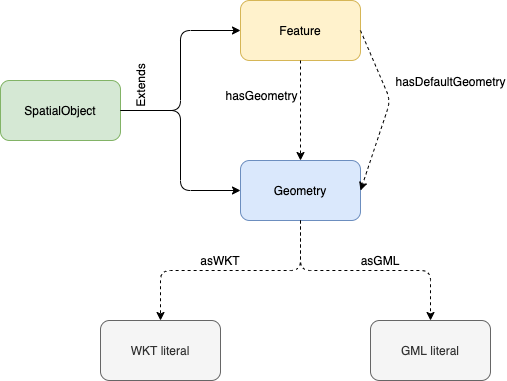
\includegraphics[width=\linewidth]{images/geosparql_architecture.png}
    \caption{Vereenvoudigd diagram van de GeoSPARQL klassen ``Feature'' en ``Geometry'' met sommige properties (figuur gebaseerd op \protect\cite{geosparqlsupport}).}
    \label{fig:abstr_geosparql_architecture}
\end{figure}

Bij GeoSPARQL is het belangrijk dat er een onderscheid wordt gemaakt tussen topologische functies en niet-topologische functies. De topologische functie beschrijven de relaties tussen objecten (bijvoorbeeld of een object in een ander object ligt), terwijl de niet-topologische functies gevarieerder zijn (bijvoorbeeld de afstand tussen twee objecten geven). 

\begin{figure}[ht]
    \centering
    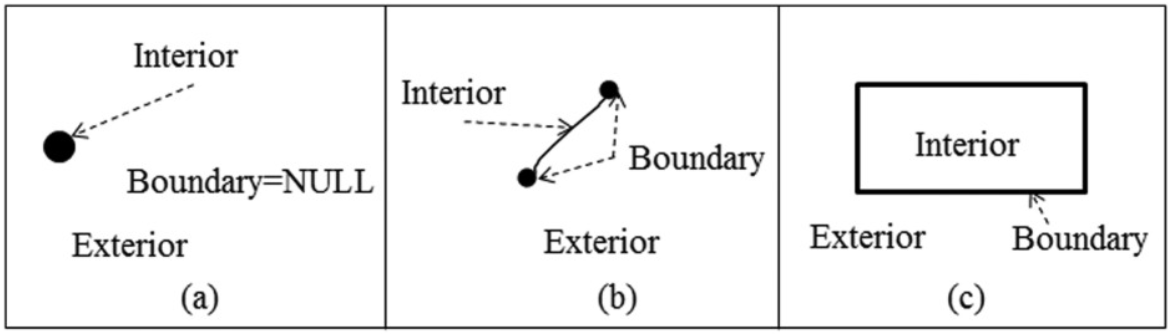
\includegraphics[width=\linewidth]{images/spatial_objects_DE-9IM.png}
    \caption{Spatiale objecten met hun \textit{interior}, \textit{boundary} en \textit{exterior}: (a) Een punt; (b) Een lijn; (c) Een vlak. Figuur van \protect\cite{shen2018classification}}.
    \label{fig:abstr_de-9im}
\end{figure}

Voor de beschrijving van topologische relaties gebruikt GeoSPARQL het DE-9IM (= \textit{Dimensionally Extended Nine-Intersection}) model. Dit model is een 3x3 matrix waarbij de \textit{interior}, \textit{boundary} en \textit{exterior} van het ene spatiale object vergeleken wordt met deze van het andere spatiale object. De betekenis van \textit{interior}, \textit{boundary} en \textit{exterior} is verduidelijkt in \figureref{fig:abstr_de-9im}. De 3x3 matrix voor twee objecten ``a'' en ``b'' is van de volgende vorm \cite{shen2018classification}:

\begin{equation*}
    DE-9IM(a,b) = 
\end{equation*}
\begin{equation*}
    \begin{bmatrix}
        dim(I(a)\cap I(b)) & dim(I(a)\cap B(b)) & dim(I(a)\cap E(b))\\
        dim(B(a)\cap I(b)) & dim(B(a)\cap B(b)) & dim(B(a)\cap E(b))\\
        dim(E(a)\cap I(b)) & dim(E(a)\cap B(b)) & dim(E(a)\cap E(b))
    \end{bmatrix}
\end{equation*}

Ten slotte voorziet GeoSPARQL ook een functionaliteit voor het herschrijven van een query. Deze is nodig wanneer een topologische functie gebruikt wordt als predikaat. Dit is nodig omdat dit enkel als predikaat bestaan wanneer dit al uitgerekend is op de server. Dit wordt niet verder aangehaald in deze masterproef aangezien de filtering op de client gebeurt, dus kan er niet uitgegaan worden van berekeningen op de server. Een ander argument om niet uit te gaan van deze berekening op de server is dat de data van verschillende bronnen kunnen komen. Dit is dus niet bruikbaar om a priori door één bron uitgerekend worden \cite{ogcdocs}.

\section{Implementatie}
Bij de implementatie van de GeoSPARQL- functionaliteiten is gebruik gemaakt van Comunica. Hier is een actor aangemaakt die de GeoSPARQL \textit{query engine} zal instantiëren. Hiervoor wordt gebruik gemaakt van ``sparqlalgebrajs'' om de SPARQL query om te vormen naar SPARQL algebra. Bovendien wordt ``sparqlee'' gebruikt om deze SPARQL algebra correct uit te voeren. Met andere woorden, ``sparqlee'' is een \textit{expression evaluator}. Bij deze implementatie zijn de effectieve GeoSPARQL-functionaliteiten dus geïmplementeerd binnen ``sparqlee''. 

Om de datastructuur van GeoSPARQL te respecteren (zie \figureref{fig:abstr_geosparql_architecture}) is gebruik gemaakt van GeoJSON. Dit is een al meer gebruikt formaat dat ondersteuning biedt voor zowel ``Geometry'' als ``Feature'' objecten. Om nu van een ``WKT literal'' naar GeoJSON te kunnen overgaan wordt gebruik gemaakt van Terraformer. 

Het volgende probleem is nu het oplossen van de topologische functies en de niet-topologische functies. Hiervoor is gebruik gemaakt van ``Turf.js''. Turf voorziet vele methoden die gebruikt kunnen worden om berekeningen te doen met geospatiale objecten. Daarnaast heeft Turf ook enkele \textit{build in} functies (zoals ``booleanContains'') die rechtstreeks gebruikt kunnen worden. Naast het functionele is Turf zo een goede keuze omdat het een grote gemeenschap heeft waardoor bugs snel gedetecteerd worden. Bovendien is Turf modulair geprogrammeerd, waardoor slechts de kleine modules die benodigd zijn ingeladen moeten worden. 

Het laatste probleem om een werkende implementatie van GeoSPARQL te bekomen is het probleem van de verschillende projecties. Dit wordt opgelost dankzij ``Proj4js''. Proj4 is een \textit{library} die zorgt voor de transformatie van coördinaten in het ene referentiesysteem naar coördinaten van het andere referentiesysteem. 

Nu een werkende implementatie van GeoSPARQL tot de beschikking is, blijft nog één implementatie onafgewerkt. Dit is een testomgeving voor het controleren welke ``Linked Data publicatie''-interfaces uitgebreid kunnen worden met GeoSPARQL-functionaliteiten. Hiervoor is gebruik gemaakt van de ``jQuery Widget'' van Comunica. Deze voorziet een grafische interface waarbij het mogelijk is om de query voortdurend aan te passen, alsook de bronnen die gebruikt worden bij deze query. Ook zal deze grafische interface zowel het bekomen resultaat visualiseren als logs weergeven. Deze logs is het meest interessante deel om deze masterproef af te toetsen. Aan de hand van deze logs kan gecontroleerd worden hoe alles intern in zijn werk gaat. 

\section{Interfaces}
Voordat begonnen kan worden met het testen van de verschillende interfaces is het nodig om een gepaste use-case te hebben. Vanwege de bekendheid is ervoor gekozen om België als use-case te nemen voor het testen. Hierbij is een oppervlakkige tekening van België gemaakt, die te zien is in \figureref{fig:abstr_demoset}. Deze tekening is gemaakt in een aangepaste schaal. Verder is deze tekening identiek (op vlak van coördinaten) aan de bijhorende dataset die terug te vinden is op GitHub Gist\footnote{https://gist.github.com/dreeki/e48bbe533a4b1191045b3652ff2c9c81}. Deze dataset is opgesplitst in vijf verschillende bestanden (namelijk: ``land'', ``gewest'', ``provincie'', ``weg'' en ``stad'') zodat deze dataset bruikbaar is voor het verifiëren of gefedereerd queryen nog steeds mogelijk is. 

\begin{figure}
    \centering
    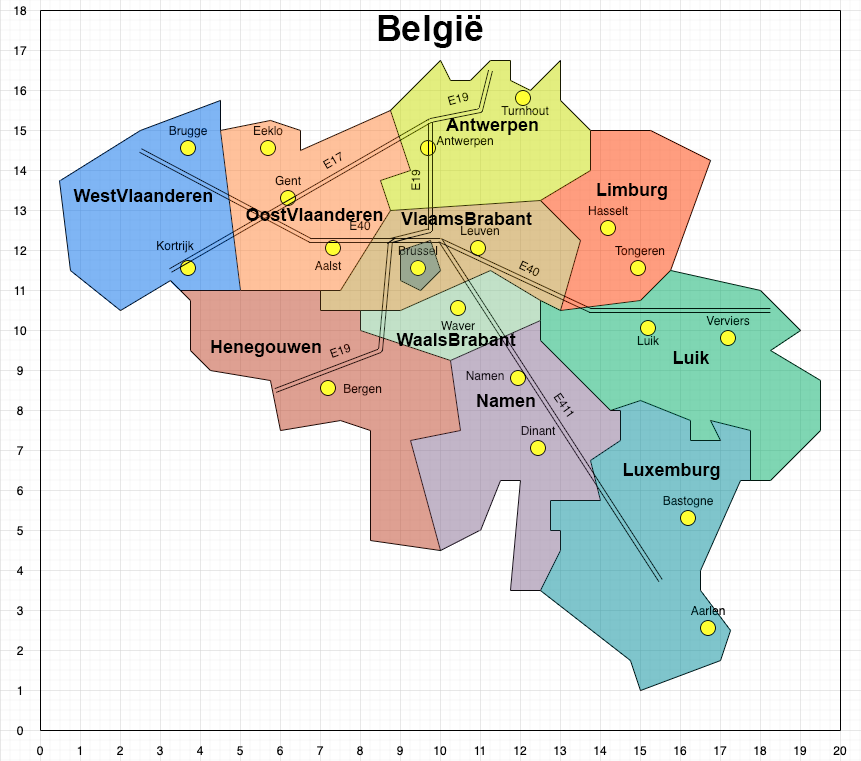
\includegraphics[width=\linewidth]{images/geosparql_demo.png}
    \caption{Testset voor het testen van de verschillende bronnen.}
    \label{fig:abstr_demoset}
\end{figure}

De eerste soort bron die gecontroleerd wordt is de ``data dump''. Deze wordt ook gebruikt als baseline omdat dit de eenvoudigste vorm is. Bij de ``data dump'' wordt de volledige dataset gedownload op de client. Op deze manier kan de client de filtering volledig uitvoeren. 

De tweede soort bron is de ``TPF interface''. Hierbij zal een server de bestanden met data beheren en antwoorden op aanvragen. Bij het queryen zal de query opgedeeld worden in verschillende \textit{triple pattern fragments}, zodat de server zelf kan beslissen om geen overbodige informatie mee te sturen. Vervolgens zal de client deze gegevens joinen zodat hij uiteindelijk het geheel kan filteren om zo de correcte resultaten te kunnen weergeven.

De derde soort bron is het ``SPARQL endpoint''. Deze is met zekerheid de moeilijke. Deze bron heeft zelf de mogelijkheid om SPARQL queries op te lossen, maar deze ondersteund zelf geen GeoSPARQL. Het is dus niet mogelijk om de GeoSPARQL query in zijn geheel door te sturen naar het ``SPARQL endpoint'' (bovendien zou gefedereerd queryen niet mogelijk zijn moest het ``SPARQL endpoint'' de query volledig zelf uitwerken). Dit probleem wordt aangepakt door de query te overlopen over zijn individuele RDF triples. Zo zal de \textit{query engine} eerst een ``count'' query maken om te weten waar het kleinst mogelijke patroon is. Dit is nodig voor een goede performantie te bekomen. De tweede stap is het effectief ophalen van dit kleinste patroon. Dit wordt meerdere malen herhaalt tot de volledige query verwerkt is. Zo wordt het geheel opnieuw gejoined op de client, zodat hier wederom de filtering kan gebeuren.

\section{Conclusie}
Om te antwoorden op de vraag welke ``Linked Data publicatie''-interfaces kunnen uitgebreid worden met GeoSPARQL-functionaliteiten door de filtering op de client uit te voeren, moeten de resultaten van voorheen geïnterpreteerd worden. 

Zo is het mogelijk om dit te doen bij ``data dumps'' doordat de client de volledige dataset download en deze vervolgens filtert. Bij ``TPF interfaces'' is dit ook mogelijk, door de verschillende \textit{triple pattern fragments} te joinen op de client. Dit resultaat kan zo ook weer gefilterd worden. Zelfs bij een ``SPARQL endpoint'' is dit mogelijk door de te tellen bij de bron hoeveel resultaten er zijn voor elk RDF triple van de query. Hierbij wordt het kleinste patroon opgehaald en gejoined op de client. Ook dit resultaat wordt opnieuw gefilterd op de client. 


\bibliographystyle{phdsymp}
%%%%%\bibliography{bib-file} % commented if *.bbl file included, as
%%%%%see below


%%%%%%%%%%%%%%%%% BIBLIOGRAPHY IN THE LaTeX file !!!!! %%%%%%%%%%%%%%%%%%%%%%%%
%% This is nothing else than the phdsymp_sample2e.bbl file that you would%%
%% obtain with BibTeX: you do not need to send around the *.bbl file  
%%
%%---------------------------------------------------------------------------%%
%
\begin{thebibliography}{1}
    \bibitem{berners2001semantic}
    Berners-Lee, Tim and Hendler, James and Lassila, Ora
    \newblock {\em The semantic web},
    \newblock Scientific american, vol. 284, no. 5, pp. 34–43, 2001.

    \bibitem{berners2006linkeddata}
    Berners Lee, Tim
    \newblock {\em Linked Data},
    \newblock 2006.

    \bibitem{lassila1998resource}
    Lassila, Ora and Swick, Ralph R and others
    \newblock {\em Resource description framework (RDF) model and syntax specification},
    \newblock 1998.

    \bibitem{heath2011linked}
    Heath, Tom and Bizer, Christian
    \newblock {\em Linked data: Evolving the web into a global data space},
    \newblock Synthesis lectures on the semantic web: theory and technology, vol. 1, no. 1, pp. 1–136, 2011.

    \bibitem{sparql2013querylanguage}
    Harris, Steve and Seaborne, Andy
    \newblock {\em SPARQL 1.1 Query Language},
    \newblock World Wide Web Consortium, 2013.

    \bibitem{taelman2018comunica}
    Taelman, Ruben and Van Herwegen, Joachim and Vander Sande, Miel and Verborgh, Ruben
    \newblock {\em Comunica: a modular SPARQL query engine for the web},
    \newblock in International Semantic Web Conference. Springer, 2018, pp. 239–255.

    \bibitem{ogcdocs}
    \newblock {\em Open Geospatial Consortium},
    \newblock URL: https://ogc.org

    \bibitem{geosparqlsupport}
    \newblock {\em GeoSPARQL support: What is GeoSPARQL},
    \newblock URL: http://graphdb.ontotext.com/documentation/standard/geosparql-support.html

    \bibitem{shen2018classification}
    Shen, Jingwei and Chen, Min and Liu, Xintao
    \newblock {\em Classification of topological relations between spatial objects in two-dimensional space within the dimensionally extended 9-intersection model},
    \newblock Transactions in GIS, vol. 22, no. 2, pp. 514–541, 2018.
\end{thebibliography}
%
%%---------------------------------------------------------------------------%%

\end{document}